%%
% Copyright (c) 2017 - 2024, Pascal Wagler;
% Copyright (c) 2014 - 2024, John MacFarlane
%
% All rights reserved.
%
% Redistribution and use in source and binary forms, with or without
% modification, are permitted provided that the following conditions
% are met:
%
% - Redistributions of source code must retain the above copyright
% notice, this list of conditions and the following disclaimer.
%
% - Redistributions in binary form must reproduce the above copyright
% notice, this list of conditions and the following disclaimer in the
% documentation and/or other materials provided with the distribution.
%
% - Neither the name of John MacFarlane nor the names of other
% contributors may be used to endorse or promote products derived
% from this software without specific prior written permission.
%
% THIS SOFTWARE IS PROVIDED BY THE COPYRIGHT HOLDERS AND CONTRIBUTORS
% "AS IS" AND ANY EXPRESS OR IMPLIED WARRANTIES, INCLUDING, BUT NOT
% LIMITED TO, THE IMPLIED WARRANTIES OF MERCHANTABILITY AND FITNESS
% FOR A PARTICULAR PURPOSE ARE DISCLAIMED. IN NO EVENT SHALL THE
% COPYRIGHT OWNER OR CONTRIBUTORS BE LIABLE FOR ANY DIRECT, INDIRECT,
% INCIDENTAL, SPECIAL, EXEMPLARY, OR CONSEQUENTIAL DAMAGES (INCLUDING,
% BUT NOT LIMITED TO, PROCUREMENT OF SUBSTITUTE GOODS OR SERVICES;
% LOSS OF USE, DATA, OR PROFITS; OR BUSINESS INTERRUPTION) HOWEVER
% CAUSED AND ON ANY THEORY OF LIABILITY, WHETHER IN CONTRACT, STRICT
% LIABILITY, OR TORT (INCLUDING NEGLIGENCE OR OTHERWISE) ARISING IN
% ANY WAY OUT OF THE USE OF THIS SOFTWARE, EVEN IF ADVISED OF THE
% POSSIBILITY OF SUCH DAMAGE.
%%

%%
% This is the Eisvogel pandoc LaTeX template.
%
% For usage information and examples visit the official GitHub page:
% https://github.com/Wandmalfarbe/pandoc-latex-template
%%

% Options for packages loaded elsewhere
\PassOptionsToPackage{unicode}{hyperref}
\PassOptionsToPackage{hyphens}{url}
\PassOptionsToPackage{dvipsnames,svgnames,x11names,table}{xcolor}
%
\documentclass[
  paper=a4,
  ,captions=tableheading
]{scrartcl}
\usepackage{amsmath,amssymb}
% Use setspace anyway because we change the default line spacing.
% The spacing is changed early to affect the titlepage and the TOC.
\usepackage{setspace}
\setstretch{1.2}
\usepackage{iftex}
\ifPDFTeX
  \usepackage[T1]{fontenc}
  \usepackage[utf8]{inputenc}
  \usepackage{textcomp} % provide euro and other symbols
\else % if luatex or xetex
  \usepackage{unicode-math} % this also loads fontspec
  \defaultfontfeatures{Scale=MatchLowercase}
  \defaultfontfeatures[\rmfamily]{Ligatures=TeX,Scale=1}
\fi
\usepackage{lmodern}
\ifPDFTeX\else
  % xetex/luatex font selection
\fi
% Use upquote if available, for straight quotes in verbatim environments
\IfFileExists{upquote.sty}{\usepackage{upquote}}{}
\IfFileExists{microtype.sty}{% use microtype if available
  \usepackage[]{microtype}
  \UseMicrotypeSet[protrusion]{basicmath} % disable protrusion for tt fonts
}{}
\makeatletter
\@ifundefined{KOMAClassName}{% if non-KOMA class
  \IfFileExists{parskip.sty}{%
    \usepackage{parskip}
  }{% else
    \setlength{\parindent}{0pt}
    \setlength{\parskip}{6pt plus 2pt minus 1pt}}
}{% if KOMA class
  \KOMAoptions{parskip=half}}
\makeatother
\usepackage{xcolor}
\definecolor{default-linkcolor}{HTML}{A50000}
\definecolor{default-filecolor}{HTML}{A50000}
\definecolor{default-citecolor}{HTML}{4077C0}
\definecolor{default-urlcolor}{HTML}{4077C0}
\usepackage[top=1.3in,bottom=1in]{geometry}
\usepackage{longtable,booktabs,array}
\usepackage{calc} % for calculating minipage widths
% Correct order of tables after \paragraph or \subparagraph
\usepackage{etoolbox}
\makeatletter
\patchcmd\longtable{\par}{\if@noskipsec\mbox{}\fi\par}{}{}
\makeatother
% Allow footnotes in longtable head/foot
\IfFileExists{footnotehyper.sty}{\usepackage{footnotehyper}}{\usepackage{footnote}}
\makesavenoteenv{longtable}
% add backlinks to footnote references, cf. https://tex.stackexchange.com/questions/302266/make-footnote-clickable-both-ways
\usepackage{footnotebackref}
\usepackage{graphicx}
\makeatletter
\newsavebox\pandoc@box
\newcommand*\pandocbounded[1]{% scales image to fit in text height/width
  \sbox\pandoc@box{#1}%
  \Gscale@div\@tempa{\textheight}{\dimexpr\ht\pandoc@box+\dp\pandoc@box\relax}%
  \Gscale@div\@tempb{\linewidth}{\wd\pandoc@box}%
  \ifdim\@tempb\p@<\@tempa\p@\let\@tempa\@tempb\fi% select the smaller of both
  \ifdim\@tempa\p@<\p@\scalebox{\@tempa}{\usebox\pandoc@box}%
  \else\usebox{\pandoc@box}%
  \fi%
}
% Set default figure placement to htbp
% Make use of float-package and set default placement for figures to H.
% The option H means 'PUT IT HERE' (as  opposed to the standard h option which means 'You may put it here if you like').
\usepackage{float}
\floatplacement{figure}{H}
\makeatother
\setlength{\emergencystretch}{3em} % prevent overfull lines
\providecommand{\tightlist}{%
  \setlength{\itemsep}{0pt}\setlength{\parskip}{0pt}}
\setcounter{secnumdepth}{-\maxdimen} % remove section numbering
\makeatletter
\@ifpackageloaded{subfig}{}{\usepackage{subfig}}
\@ifpackageloaded{caption}{}{\usepackage{caption}}
\captionsetup[subfloat]{margin=0.5em}
\AtBeginDocument{%
\renewcommand*\figurename{Figura}
\renewcommand*\tablename{Tabla}
}
\AtBeginDocument{%
\renewcommand*\listfigurename{Lista de Figuras}
\renewcommand*\listtablename{Lista de Tablas}
}
\newcounter{pandoccrossref@subfigures@footnote@counter}
\newenvironment{pandoccrossrefsubfigures}{%
\setcounter{pandoccrossref@subfigures@footnote@counter}{0}
\begin{figure}\centering%
\gdef\global@pandoccrossref@subfigures@footnotes{}%
\DeclareRobustCommand{\footnote}[1]{\footnotemark%
\stepcounter{pandoccrossref@subfigures@footnote@counter}%
\ifx\global@pandoccrossref@subfigures@footnotes\empty%
\gdef\global@pandoccrossref@subfigures@footnotes{{##1}}%
\else%
\g@addto@macro\global@pandoccrossref@subfigures@footnotes{, {##1}}%
\fi}}%
{\end{figure}%
\addtocounter{footnote}{-\value{pandoccrossref@subfigures@footnote@counter}}
\@for\f:=\global@pandoccrossref@subfigures@footnotes\do{\stepcounter{footnote}\footnotetext{\f}}%
\gdef\global@pandoccrossref@subfigures@footnotes{}}
\@ifpackageloaded{float}{}{\usepackage{float}}
\floatstyle{ruled}
\@ifundefined{c@chapter}{\newfloat{codelisting}{h}{lop}}{\newfloat{codelisting}{h}{lop}[chapter]}
\floatname{codelisting}{Listing}
\newcommand*\listoflistings{\listof{codelisting}{Listas del Documento}}
\makeatother
\usepackage{bookmark}
\IfFileExists{xurl.sty}{\usepackage{xurl}}{} % add URL line breaks if available
\urlstyle{same}
\hypersetup{
  pdftitle={Propuesta de Certificación Operativa Plataforma de Software Trii.co (borrador)},
  pdfsubject={Implementación Proyecto},
  pdfkeywords={Rendimiento, Métodos pruebas, Pruebas software, QA},
  hidelinks,
  breaklinks=true,
  pdfcreator={LaTeX via pandoc with the Eisvogel template}}
\title{Propuesta de Certificación Operativa Plataforma de Software
Trii.co (borrador)}
\usepackage{etoolbox}
\makeatletter
\providecommand{\subtitle}[1]{% add subtitle to \maketitle
  \apptocmd{\@title}{\par {\large #1 \par}}{}{}
}
\makeatother
\subtitle{Borrador}
\author{}
\date{2025-01-15}



%%
%% added
%%


%
% for the background color of the title page
%

%
% break urls
%
\PassOptionsToPackage{hyphens}{url}

%
% When using babel or polyglossia with biblatex, loading csquotes is recommended
% to ensure that quoted texts are typeset according to the rules of your main language.
%
\usepackage{csquotes}

%
% captions
%
\definecolor{caption-color}{HTML}{777777}
\usepackage[font={stretch=1.2}, textfont={color=caption-color}, position=top, skip=4mm, labelfont=bf, singlelinecheck=false, justification=raggedright]{caption}
\setcapindent{0em}

%
% blockquote
%
\definecolor{blockquote-border}{RGB}{221,221,221}
\definecolor{blockquote-text}{RGB}{119,119,119}
\usepackage{mdframed}
\newmdenv[rightline=false,bottomline=false,topline=false,linewidth=3pt,linecolor=blockquote-border,skipabove=\parskip]{customblockquote}
\renewenvironment{quote}{\begin{customblockquote}\list{}{\rightmargin=0em\leftmargin=0em}%
\item\relax\color{blockquote-text}\ignorespaces}{\unskip\unskip\endlist\end{customblockquote}}

%
% Source Sans Pro as the default font family
% Source Code Pro for monospace text
%
% 'default' option sets the default
% font family to Source Sans Pro, not \sfdefault.
%
\ifnum 0\ifxetex 1\fi\ifluatex 1\fi=0 % if pdftex
    \usepackage[default]{sourcesanspro}
  \usepackage{sourcecodepro}
  \else % if not pdftex
    \usepackage[default]{sourcesanspro}
  \usepackage{sourcecodepro}

  % XeLaTeX specific adjustments for straight quotes: https://tex.stackexchange.com/a/354887
  % This issue is already fixed (see https://github.com/silkeh/latex-sourcecodepro/pull/5) but the
  % fix is still unreleased.
  % TODO: Remove this workaround when the new version of sourcecodepro is released on CTAN.
  \ifxetex
    \makeatletter
    \defaultfontfeatures[\ttfamily]
      { Numbers   = \sourcecodepro@figurestyle,
        Scale     = \SourceCodePro@scale,
        Extension = .otf }
    \setmonofont
      [ UprightFont    = *-\sourcecodepro@regstyle,
        ItalicFont     = *-\sourcecodepro@regstyle It,
        BoldFont       = *-\sourcecodepro@boldstyle,
        BoldItalicFont = *-\sourcecodepro@boldstyle It ]
      {SourceCodePro}
    \makeatother
  \fi
  \fi

%
% heading color
%
\definecolor{heading-color}{RGB}{40,40,40}
\addtokomafont{section}{\color{heading-color}}
% When using the classes report, scrreprt, book,
% scrbook or memoir, uncomment the following line.
%\addtokomafont{chapter}{\color{heading-color}}

%
% variables for title, author and date
%
\usepackage{titling}
\title{Propuesta de Certificación Operativa Plataforma de Software
Trii.co (borrador)}
\author{}
\date{2025-01-15}

%
% tables
%

\definecolor{table-row-color}{HTML}{F5F5F5}
\definecolor{table-rule-color}{HTML}{999999}

%\arrayrulecolor{black!40}
\arrayrulecolor{table-rule-color}     % color of \toprule, \midrule, \bottomrule
\setlength\heavyrulewidth{0.3ex}      % thickness of \toprule, \bottomrule
\renewcommand{\arraystretch}{1.3}     % spacing (padding)


%
% remove paragraph indentation
%
\setlength{\parindent}{0pt}
\setlength{\parskip}{6pt plus 2pt minus 1pt}
\setlength{\emergencystretch}{3em}  % prevent overfull lines

%
%
% Listings
%
%


%
% header and footer
%
\usepackage[headsepline,footsepline]{scrlayer-scrpage}

\newpairofpagestyles{eisvogel-header-footer}{
  \clearpairofpagestyles
  \ihead*{2025-01-15}
  \chead*{}
  \ohead*{Propuesta de Certificación Operativa Plataforma de Software
Trii.co (borrador)}
  \ifoot*{}
  \cfoot*{}
  \ofoot*{\thepage}
  \addtokomafont{pageheadfoot}{\upshape}
}
\pagestyle{eisvogel-header-footer}



%%
%% end added
%%

\begin{document}

%%
%% begin titlepage
%%

%%
%% end titlepage
%%

% \maketitle


\subsection{Control de Cambios}\label{sec:control-de-cambios}

Historia de cambiod de la propuesta.

\section{Descripción de la
Propuesta}\label{sec:descripciuxf3n-de-la-propuesta}

Informe de refrendo operativo de la plataforma Trii.co mediante plan de
pruebas de rendimiento de software consignados en la actual propuesta.

\section{Detalles Técnicos de la
Propuesta}\label{sec:detalles-tuxe9cnicos-de-la-propuesta}

Esta propuesta contienen los siguientes componentes técnicos.

\begin{itemize}
\tightlist
\item
  Metas del proyecto e interesados
\item
  Alcance
\item
  Métodos
\item
  Entregables
\item
  Plan de Trabajo y cronograma propuesto
\item
  Consideraciones, costos y restricciones
\end{itemize}

\subsection{Metas de la Propuesta}\label{sec:metas-de-la-propuesta}

\begin{enumerate}
\def\labelenumi{\arabic{enumi}.}
\tightlist
\item
  En cuanto al método de la propuesta: presentar un plan de pruebas de
  rendimiento suficiente y acotado a la corroboración operativa en
  términos de rendimiento exigida a la plataforma Trii.co
\item
  En cuanto a la necesidad: alinear el plan de pruebas de rendimiento
  con los condiciones requeridas de tiempo y entregables resultantes con
  las exigencias de los interesados de la propuesta
\end{enumerate}

\subsection{Alcance}\label{sec:alcance}

\begin{enumerate}
\def\labelenumi{\arabic{enumi}.}
\tightlist
\item
  Planificación. Período inicial de definición y acuerdos de los
  objetivos puntuales de las pruebas de rendimiento de la plataforma
  Trii.co.
\item
  Preparación. Lista de chequeo de estado de los entornos de trabajo
  disponibles de la plataforma Trii.co: hardware, software, redes,
  accesos, y permisos/equipo de trabajo.
\item
  Alistamiento. Chequeo del estado y disponibilidad del plano de datos
  de entrada y de los recursos disponibles de las pruebas.
\item
  Definición. Confirmación del diseño de los escenarios del tipo de
  pruebas consignadas en la propuesta. Identificación de otras
  dependencias.
\item
  Verificación. Establecer los criterios y umbrales de aceptación del
  tipo de pruebas consignadas en la propuesta.
\item
  Ejecución. Aseguramiento y ejecución del plan de pruebas consignado en
  esta propuesta.
\item
  Alineación. Contrastar el resultado de las pruebas consignadas en esta
  propuesta con las metas también aquí definidas.
\end{enumerate}

\subsection{Exclusiones del Alcance}\label{sec:exclusiones-del-alcance}

La presenta propuesta no incluye:

\begin{enumerate}
\def\labelenumi{\arabic{enumi}.}
\tightlist
\item
  Por restricciones de tiempo, la actual propuesta no incluye análisis
  ni recomendaciones de diseño/arquitectura
\item
  No incluye plan de capacidad / proyección de uso infraestructura
  futura
\end{enumerate}

\subsection{Métodos Propuestos}\label{sec:muxe9todos-propuestos}

Lista de métodos aplicables a la propuesta seleccionados en función de
los objetivos trazados.

\begin{enumerate}
\def\labelenumi{\arabic{enumi}.}
\tightlist
\item
  Marco de Trabajo Proceso de Pruebas Ágiles Testfully
\item
  Método de Pruebas en V (v-model): Verificación y Validación
\item
  Técnicas de Pruebas Dinámicas
\item
  Tipo de Pruebas: no funcionales
\item
  Alineación Comprobable de Criterios de Interesados
\item
  Aplicación del Principio de Observabilidad
\item
  Resultados de Prueba de Una-Página
\end{enumerate}

\subsection{Entregables de la
Propuesta}\label{sec:entregables-de-la-propuesta}

\begin{enumerate}
\def\labelenumi{\arabic{enumi}.}
\tightlist
\item
  Informe de línea base del rendimiento de la plataforma Trii.co/
\item
  Informe ejecutivo de refrendo de la plataforma Trii.co.
\item
  Informe técnico de las pruebas de rendimiento de la plataforma
  Trii.co.
\end{enumerate}

\subsection{Plan de Trabajo}\label{sec:plan-de-trabajo}

\begin{enumerate}
\def\labelenumi{\arabic{enumi}.}
\tightlist
\item
  Planificación, 4 hrs
\item
  Preparación, 4 hrs
\item
  Alistamiento, 8 hrs o menos (*)
\item
  Definición, 8 hrs (*)
\item
  Verificación, 4 hrs
\item
  Ejecución, 16 hrs
\item
  Alineación, 8 hrs
\end{enumerate}

\begin{figure}
\centering
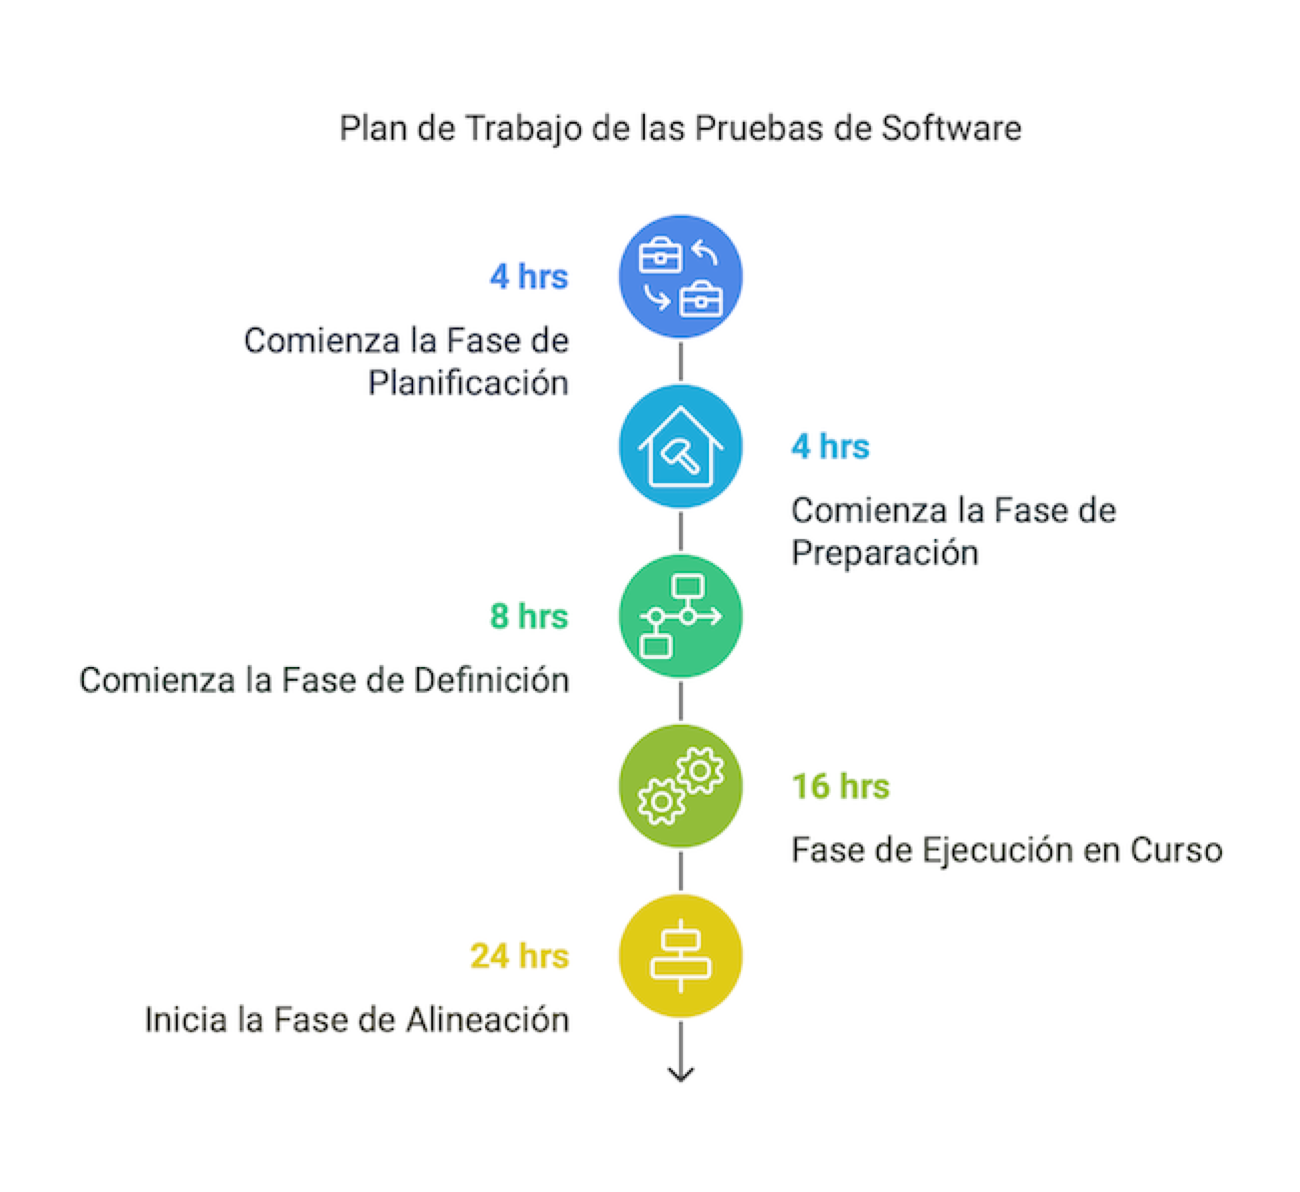
\includegraphics{images/plan.png}
\caption{Plan de Trabajo Propuesta Pruebas Plataforma
Trii.co}\label{fig:plan}
\end{figure}

\subsubsection{Cronograma de Ejecución del
Plan}\label{sec:cronograma-de-ejecuciuxf3n-del-plan}

\begin{figure}
\centering
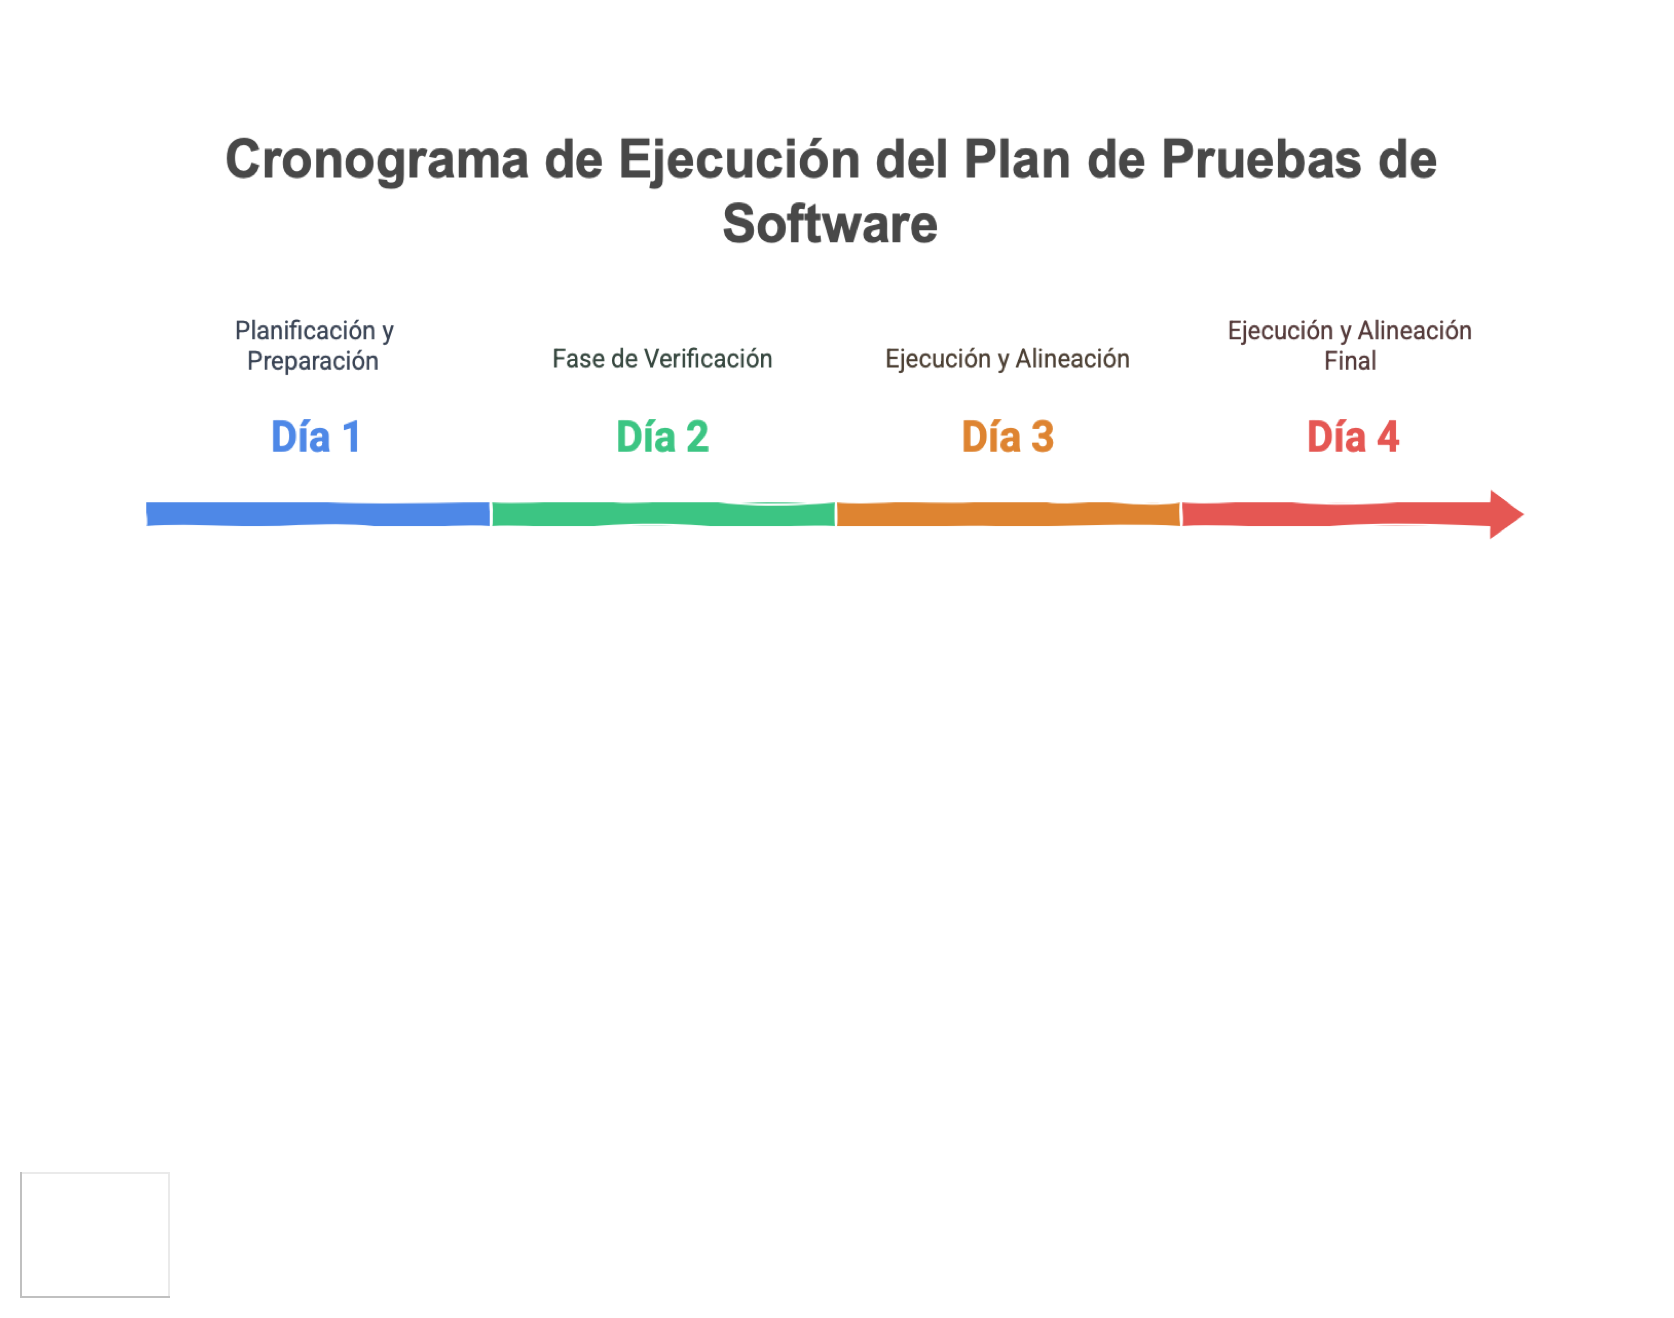
\includegraphics{images/cronograma.png}
\caption{Cronograma Propuesta Pruebas Plataforma
Trii.co}\label{fig:cronograma}
\end{figure}

1er día, actividades en paralelo - Planificación, 4 hrs - Preparación. 4
hrs - Alistamiento. 8 hrs o menos (*)

2do día, actividades en paralelo - Definición. 8 hrs (*) - Verificación.
4 hrs

3er día, actividades en paralelo - Ejecución. 8 hrs - Alineación. 4 hrs

4to día, actividades en paralelo - Ejecución. 8 hrs - Alineación. 4 hrs

\subsection{Propuesta Económica}\label{sec:propuesta-econuxf3mica}

La presente propuesta, en los términos consignados aquí, presenta el
costo de

\begin{longtable}[]{@{}
  >{\raggedright\arraybackslash}p{(\columnwidth - 4\tabcolsep) * \real{0.6974}}
  >{\raggedright\arraybackslash}p{(\columnwidth - 4\tabcolsep) * \real{0.1579}}
  >{\raggedright\arraybackslash}p{(\columnwidth - 4\tabcolsep) * \real{0.1447}}@{}}
\toprule\noalign{}
\begin{minipage}[b]{\linewidth}\raggedright
Ítem
\end{minipage} & \begin{minipage}[b]{\linewidth}\raggedright
Costo
\end{minipage} & \begin{minipage}[b]{\linewidth}\raggedright
Impuestos
\end{minipage} \\
\midrule\noalign{}
\endhead
\bottomrule\noalign{}
\endlastfoot
Definición, ejecución y entregables plan de pruebas & \$1.150 USD &
Sí \\
\end{longtable}

Nota: los valores del costo de la propuesta se mantienen durante los
siguientes 3 días laborales luego de su presentación a los interesados.

\subsection{Forma de Pago de la
Propuesta}\label{sec:forma-de-pago-de-la-propuesta}

\begin{longtable}[]{@{}lll@{}}
\toprule\noalign{}
Pagos & Fracción & Hito del Plan \\
\midrule\noalign{}
\endhead
\bottomrule\noalign{}
\endlastfoot
Primer pago & 50\% & Planificación, Preparación \\
Segundo pago & 50\% & Ejecución \\
\end{longtable}

\subsection{Equipo de Trabajo}\label{sec:equipo-de-trabajo}

\begin{longtable}[]{@{}
  >{\raggedright\arraybackslash}p{(\columnwidth - 6\tabcolsep) * \real{0.5063}}
  >{\raggedright\arraybackslash}p{(\columnwidth - 6\tabcolsep) * \real{0.0886}}
  >{\raggedright\arraybackslash}p{(\columnwidth - 6\tabcolsep) * \real{0.1899}}
  >{\raggedright\arraybackslash}p{(\columnwidth - 6\tabcolsep) * \real{0.2152}}@{}}
\toprule\noalign{}
\begin{minipage}[b]{\linewidth}\raggedright
Recurso
\end{minipage} & \begin{minipage}[b]{\linewidth}\raggedright
Cant.
\end{minipage} & \begin{minipage}[b]{\linewidth}\raggedright
Participación
\end{minipage} & \begin{minipage}[b]{\linewidth}\raggedright
Observaciones
\end{minipage} \\
\midrule\noalign{}
\endhead
\bottomrule\noalign{}
\endlastfoot
Especialista encargado plan de pruebas & 1 & 100\% & \\
Ingeniero apoyo a las pruebas & 1 & 2 días & Interno cliente \\
\end{longtable}

Nota: por las restricciones de ejecución conocidas al momento de la
realización de esta propuesta es requerido un apoyo interno de la
empresa cliente Trii.co con la participación indicada en la tabla.

\subsection{Consideraciones Generales de la
Propuesta}\label{sec:consideraciones-generales-de-la-propuesta}

\begin{enumerate}
\def\labelenumi{\arabic{enumi}.}
\tightlist
\item
  Forma de pago de la propuesta: 50\% al inicio, 50\% al final,
  contraentrega.
\item
  Por las restricciones propias de proyecto, requiere apoyo de un
  ingeniero interno de la empresa, dedicado el 50\% de la duración del
  plan.
\item
  Las estimaciones de costo, esfuerzo, tiempo, y planeación son
  aproximadas, y representan la intención de la propuesta con la
  información conocida por las partes al momento de su realización.
\item
  Las extensiones en los entregables, o cambios a la propuesta se
  acordarán en definición y extensión por separado.
\item
  La tarifa de los controles de cambio de la propuesta es de \$/.
  120.000 COP la hora. Incluye impuestos.
\end{enumerate}

\section{Resumen de Propuesta de Certificación Operativa Plataforma de
Software de la Plataforma
Trii.co}\label{sec:resumen-de-propuesta-de-certificaciuxf3n-operativa-plataforma-de-software-de-la-plataforma-trii.co}

\begin{itemize}
\tightlist
\item
  4 días trabajo
\item
  Requiere apoyo de un ingeniero interno de la empresa, dedicado dos
  días
\item
  El resultado son 3 informes: línea base, ejecutivo, y técnico.
\item
  Costo es de \$1150 USD, con impuestos.
\item
  No incluye: por restricciones de tiempo no incluye recomendaciones de
  diseño/arquitectura, ni plan de capacidad proyección de uso
  infraestructura
\end{itemize}

\end{document}
